\documentclass[a4paper,oneside,11pt,DIV12,headsepline,footexclude,headexclude]{scrartcl}


%% Normal LaTeX or pdfLaTeX? %%%%%%%%%%%%%%%%%%%%%%%%%%%%%%%%
%% ==> The new if-Command "\ifpdf" will be used at some
%% ==> places to ensure the compatibility between
%% ==> LaTeX and pdfLaTeX.
\newif\ifpdf
\ifx\pdfoutput\undefined
	\pdffalse              %%normal LaTeX is executed
\else
	\pdfoutput=1
	\pdftrue               %%pdfLaTeX is executed
\fi

%% Packages for Graphics & Figures %%%%%%%%%%%%%%%%%%%%%%%%%%
\ifpdf %%Inclusion of graphics via \includegraphics{file}
	\usepackage[pdftex]{graphicx} %%graphics in pdfLaTeX
\else
	\usepackage[dvips]{graphicx} %%graphics and normal LaTeX
\fi
\graphicspath{{fig/}}

%% Fonts for pdfLaTeX %%%%%%%%%%%%%%%%%%%%%%%%%%%%%%%%%%%%%%%
%% ==> Only needed, if cm-super-fonts are not installed
%\ifpdf
	%\usepackage{ae}       %%Use only just one of these packages:
	%\usepackage{zefonts}  %%depends on your installation.
%\else
	%%Normal LaTeX - no special packages for fonts required
%\fi

\renewcommand{\rmdefault}{pbk} % bookman
\renewcommand{\sfdefault}{phv} % helvetica (avantgarde = pag)
\renewcommand{\ttdefault}{pcr} % courier
\renewcommand{\familydefault}{phv}

%\usepackage{cmbright}  % computer modern bright - not for pdf


\areaset{16cm}{24cm}
\addtolength{\topskip}{0.5cm}


% texttt hyphenation
\newcommand{\origttfamily}{}
\let\origttfamily=\ttfamily
\renewcommand{\ttfamily}{\origttfamily \hyphenchar\font=`\-}


\usepackage[T1]{fontenc}
\usepackage[latin1]{inputenc}
\usepackage{array}
\usepackage{float}
\usepackage{amssymb}
\usepackage{listings}
\usepackage{svg}
\usepackage[hidelinks]{hyperref}
\usepackage{paralist}
\usepackage{amsmath}
\usepackage{color}

\usepackage{listings}
\lstset{language=Java,basicstyle=\ttfamily\small,tabsize=2}


%% Line Spacing %%%%%%%%%%%%%%%%%%%%%%%%%%%%%%%%%%%%%%%%%%%%%
%\usepackage{setspace}
%\singlespacing        %% 1-spacing (default)
%\onehalfspacing       %% 1,5-spacing
%\doublespacing        %% 2-spacing

\linespread{1.05}
\addtolength{\parskip}{0.175\baselineskip}

\widowpenalty = 10000
\clubpenalty = 10000


%%%%%%%%%%%%%%%%%%%%%%%%%%%%%%%%%%%%%%%%%%%%%%%%%%%%%%%%%%%%%
%% DOCUMENT
%%%%%%%%%%%%%%%%%%%%%%%%%%%%%%%%%%%%%%%%%%%%%%%%%%%%%%%%%%%%%
\begin{document}

%% File Extensions of Graphics %%%%%%%%%%%%%%%%%%%%%%%%%%%%%%
%% ==> This enables you to omit the file extension of a graphic.
%% ==> "\includegraphics{title.eps}" becomes "\includegraphics{title}".
%% ==> If you create 2 graphics with same content (but different file types)
%% ==> "title.eps" and "title.pdf", only the file processable by
%% ==> your compiler will be used.
%% ==> pdfLaTeX uses "title.pdf". LaTeX uses "title.eps".
\ifpdf
	\DeclareGraphicsExtensions{.pdf,.jpg,.png}
\else
	\DeclareGraphicsExtensions{.eps}
\fi


\pagestyle{plain} %Now display headings: headings / fancy / ...

\title{\Huge Group 5 Lab Report}
\subtitle{\Large Solving the Convex Hull problem with CUDA}
\author{Michele Tamborrino, Technische Universit{\"a}t Wien\\
Marco Stabile, Technische Universit{\"a}t Wien\\
Gabriele Cimador, Technische Universit{\"a}t Wien\\
Evelina Eremia, Technische Universit{\"a}t Wien}
\date{} %%If commented, the current date is used.

\maketitle

\[\rule{135mm}{.5mm}\]
\begin{section}{Introduction}
 In various fields such as computer graphics, pattern recognition, and image processing it is crucial sometimes to find the smallest convex set that contains a group of points. It is not an easy task, all the more so if the set of points is in space with dimensions more than 2. But for the latter case, there are some algorithms that provide a good solution to this geometrical problem. Nevertheless this computation may be computational-heavy, as much as the input points increase in number. This is the reason why this project aims to offer a solution based on parallelization using GPUs\footnote{Graphics Processing Unit} and the CUDA\footnote{Compute Unified Device Architecture} framework, developed by NVIDIA. By offloading computationally intensive tasks to the GPU, we expect to achieve significant performance improvements over traditional CPU-based implementations.
 \subsection{The Algorithm}
 The QuickHull algorithm is an efficient method for computing the convex hull of a set of points in two-dimensional or three-dimensional space. The main idea is to identify the extreme points, which are the points located on the boundaries of the convex hull, and construct a portion of the hull between them. Subsequently, the algorithm recursively divides the point set into two subsets, one on each side of the line connecting the two extreme points. This process continues until all points are included in the convex hull. The QuickHull algorithm exploits the concept of "divide and conquer" to achieve its efficient computational complexity. The first iteration takes two points called \(P\) and \(Q\) that are defiintely on the hull and draw the line \(PQ\), then all the points above the line clockwise are kept and the farthest point \(F\) among them is searched.
 \begin{figure}[h!]
     \centering
     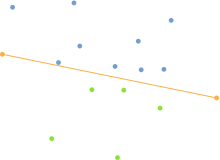
\includegraphics[width=0.5\textwidth]{img/220px-Quickhull_example3.svg.png}
     \caption{First iteration.}
     \label{pq}
 \end{figure}
 \newpage
 Once it is found, the following iterations continue with \(FP\) and \(PQ\) respectively.
  \begin{figure}[h!]
     \centering
     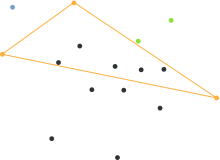
\includegraphics[width=0.5\textwidth]{img/220px-Quickhull_example6.svg.png}
     \caption{Second and third iteration.}
     \label{pq}
 \end{figure}
\end{section}
\begin{section}{Development}
For the project \href{https://www.nvidia.com/en-us/data-center/tesla-t4/}{NVIDIA T4} is used via ssh. The code has been developed locally on students' pc and run on the GPU mentioned before. The programming language used is obviously C++ to easily take advantage the CUDA framework and the complete source code is available at the following \href{https://github.com/cima22/CUDA_PlanarConvexHull/tree/main}{GitHub repository}.
\subsection{Header file}
To first block of the code is the header file, where the characteristics of the Point variable are specified and some other useful parameters, such as the seed for the random generator and how many points are desired as input. This simple file promotes simplicity of use and parameterised code.
\lstset{language=C++}
\begin{lstlisting}[caption={Header file.}, captionpos=b]
#ifndef GPU_RANDOM_POINTS_H
#define GPU_RANDOM_POINTS_H

#include <vector>

struct Point {
    double x;
    double y;
};

std::vector<Point> generate_random_points();

const int N = 2000;
const int RANGE = 300;

static unsigned int seed = 2023;

#endif //GPU_RANDOM_POINTS_H
\end{lstlisting}
In this way whenever the input size, the range or the dimension of points have to be change, it would only require minor changes in this file and compile again.
\subsection{Points generator}
For the generation of points there is a separate cpp file called \textbf{points\_generator.cpp} that uses the random library to populate an std vector, and then return it to the caller.
\lstset{language=C++}
\begin{lstlisting}[caption={Random points generator.}, captionpos=b]
#include <vector>
#include <random>
#include "random_points.h"

std::vector<Point> generate_random_points() {
    std::mt19937 rng(seed);
    std::uniform_real_distribution<double> dist(-RANGE, RANGE);

    std::vector<Point> points(N);
    for (int i = 0; i < N; i++) {
        points[i].x = dist(rng);
        points[i].y = dist(rng);
    }

    return points;
}

\end{lstlisting}
\subsection{Sequential code}
Performance evaluations cannot be done without a benchmark. Therefore the first actual program is a sequential one. Basically it implement the QuickHull Algorithm using recursion. The first iteration finds the point \(F\) and for all the consecutive calls another function is invoked, but with the same name. 
\lstset{language=C++}
\begin{lstlisting}[caption={Function in sequential program.}, captionpos=b]
// QuickHull algorithm
std::vector<Point> quickHull(const std::vector<Point>& v) {
    std::vector<Point> hull;
    auto by_x = [](const Point& p1, const Point& p2){
        return (p1.x < p2.x || (p1.x == p2.x && p1.y < p2.y));
    };
    // Start with the leftmost and rightmost points.
    Point p = *std::min_element(v.begin(), v.end(), by_x);
    Point q = *std::max_element(v.begin(), v.end(), by_x);

    // Split the points on either side of segment (a, b)
    std::vector<Point> left, right;
    for (auto t : v) {
        switch (isAboveClockwise(p, q, t)) {
            case above:
                left.push_back(t);
                break;
            case below:
                right.push_back(t);
                break;
            case on:
                break;
        }
    }

    // Be careful to add points to the hull
    // in the correct order. Add our leftmost point.
    hull.push_back(p);

    // Add hull points from the left (top)
    quickHull(left, p, q, hull);

    // Add our rightmost point
    hull.push_back(q);

    // Add hull points from the right (bottom)
    quickHull(right, q, p, hull);

    return hull;
}
\end{lstlisting}
The entire code is not reported otherwise the report would be too long.
\subsection{Parallelized code with CUDA}
For the project 5 version of CUDA programs have been developed:
\begin{enumerate}
    \item[$\blacksquare$] a first version of parallelized code with classic memory usage.

    \item[$\blacksquare$] A second version that uses the Pinned Memory standard.
\\
    \item[$\blacksquare$] A third version that uses Zero-Copy Memory, which is of course pinned.
\\
    \item[$\blacksquare$] A fourth version that uses the Unified Memory.
\\
    \item[$\blacksquare$] A fifth version that exploits the thrust library, well known for its simplicity.
\end{enumerate}
In the following chapter each program will be tested and compared in execution time with the sequential code, with some parameters changed, such as the input sizes.
\end{section}
\begin{section}{Performance Evaluations}
In this chapter we are going to compare CPU and GPU code and see if there are any differences in execution time and number of inputs. After that, also the different versions of GPU code will be compard one another to obtain an insight on how a GPU and a parallelized code can perform.
\subsection{CPU vs GPU}
The first comparison is done with CPU and GPU with classical memory usage and thread block size equal to 256. The running times are average values over 5 iteration of the respective program. It is clear in Fig.\ref{cpuvsgpu} that GPUs are not champion in computing power but in throughput: for lower sets of points, the CPU still stands a chance whereas for larger sets its execution time increases drastically. On the other hand, GPU's running times are quite the same for every set, meaning that it is totally worth an intensive usage of its resources.
\begin{figure}[H]
    \centering
    \includesvg[width=\textwidth]{img/cpugpu.svg}
    \caption{Average running times of CPU and GPU with fixed block size of 256 and changing input points number.}
    \label{cpuvsgpu}
\end{figure}
This also means that over a certain threshold GPU is the only solution for some tasks, as we can see with 20 million points performance.
To highlight the last case, it is useful to compute the absolute speed up:
\begin{equation*}
    S_{a}=\frac{T_{seq}}{T_{par}}=\frac{2654523\ \mu s}{319454\ \mu s}=8
\end{equation*}
which is an impressive speed-up for such a problem, but take into account that an absolute speed-up alone is not enough to do deep performance considerations.
\subsection{Different GPU's implementations}
CUDA's framework provides different approches when accessing and using memory of a GPU, which can improve or worsen the overall performances. For this reason this project aim to test several implementatio and not rely on only one to have a more general view and a deeper understanding. In addition to the first version, we have:
\begin{enumerate}
    \item[$\blacksquare$] \textbf{pinned\_quickhull.cu} uses the Pinned Memory approach. Basically it avoids the creattion of a pageable memory.

    \item[$\blacksquare$] \textbf{zero\_quickhull.cu} uses the Zero-Copy Memory, allowing host and device to access each other's variables.
\\
    \item[$\blacksquare$] \textbf{unified\_quickhull.cu} uses the Unified Memory, to avoid distinction between host and device pointers.
\\
    \item[$\blacksquare$]  \textbf{thrust\_quickhull.cu}, where Thrust library has been used.
\end{enumerate}
In the following figure \ref{gpus} it is possible to see each performance compared.
\begin{figure}[H]
    \centering
    \includesvg[width=\textwidth]{img/gpus.svg}
    \caption{Performances of different implementations.}
    \label{gpus}
\end{figure}
This plot needs some comments. For 2000 points in input all implementations the slowest implementations is the one with thrust, which is the price to pay for simplicity, while the fastest is the one with Pinned Memory with just \(41\mu s\). The other versions are quite comparable. In the second test with 20000 points the classic, Zero-Copy and Thurst implementations increased, while Unified did not by a lot. Zero-Copy version got slower of almost 10 times, whereas thee Pinned version is still the best. In the last case the Zero-Copy's time increased drastically, whereas the classic version did not change. Thrust implementation got slower but it can still be a good choice when simplicity is the most important factor for the developer. In the end, the best program is the one using the Pinned Memory. Nevertheless, it is important to highlight that these considerations may be true when talking about the convex hull problem, but might be false for any other problem. The context and the style of the implementation matters.
\subsection{The relevance of Thread Block Size}
Another important factor for performances is the block size. The block size in CUDA programming plays a crucial role in achieving efficient and optimal GPU utilization. The block size determines how many threads are executed together on a single CUDA block.
The choice of block size impacts several aspects of CUDA execution, including memory access patterns, thread synchronization, and occupancy. Choosing the right block size involves considering factors such as the problem size, memory requirements, and hardware constraints. A block size that is too small may result in underutilization of the GPU, while a block size that is too large may lead to resource wastage and decreased performance. This is the reason why it is useful to test different block sizes. Now take in consideration the fastest program and change its default block size to see wheter an additional improvement is possible.
\begin{figure}[H]
    \centering
    \includesvg[width=\textwidth]{img/bs.svg}
    \caption{Pinned Memory's execution times with different block sizes.}
    \label{bs}
\end{figure}
It stands out that a poor choice, for example 1 thread per block, can lead to a way higher running time even with a cool code. Regarding the other sizes, they are similar but it turns out the default size we chose was not even the better one. Therefore the program using pinned memory can get faster if a block size of 64 is set.
\end{section}
\newpage
\begin{section}{Conclusions}
In conclusion, our project involved developing a CUDA implementation for solving the Convex Hull problem exploiting the Quickhull algorithm, leveraging the parallel processing capabilities of GPUs. Throughout the project, we observed significant performance improvements compared to a CPU-based implementation when the input size is big enough. Thanks to the theory of GPU's architecture it has been easier to get hands on the code and provide a reasonable solution to thee geometrical problem.
\subsection{Lesson learnt}
Throughout this project, we gained valuable experience in utilizing CUDA for memory allocation and data transfer between the CPU and GPU, leveraging various memory standards such as pinned memory, zero copy, and unified memory.
We learned how to effectively allocate memory on the GPU using CUDA APIs, ensuring efficient data movement and minimizing data transfer overhead. Pinned memory allowed us to achieve faster data transfers by eliminating page faults, while zero copy memory enabled direct access to host memory from the GPU, avoiding explicit data transfers.
Moreover, we explored the concept of unified memory, which provided a simplified programming model by automatically managing data movement between the CPU and GPU. This allowed us to focus more on algorithm design and less on explicit memory management.
In addition to memory-related aspects, we acquired knowledge in developing CUDA kernels to perform specific tasks. We learned to carefully select the appropriate thread indices and coordinate their execution to maximize parallelism and achieve optimal performance.Furthermore, we gained proficiency in compiling and running CUDA code, understanding the compilation process and utilizing the necessary compiler flags and runtime configurations.
\subsection{Open issues}
As we moved forward in this project, we encountered two pitfalls with the CUDA programs, except for the Thrust one. The first issue is the potential presence of duplicates points in the result vector, even though the kernel follows the theoretical quickhull algorithm. On the other hand, the results of Thurst program and squential program are reasonable and consistent. The second issue is a likely segmentation fault error when the input points are 2 millions or more for some of the executables.  
\subsection{Future works}
In terms of future works, it would be valuable to address the two open issues we encountered during the project. First, solving the potential duplication of points in the resulting vector when using CUDA versions other than Thrust. Second, optimizing the memory allocation strategy to handle segmentation faults when dealing with a large number of starting points. Additionally, it would be an interesting avenue for further development exploring and testing versions of the algorithm that handle three-dimensional points and beyond, since modern-life problems would require a solution of this kind.
\end{section}
\end{document}
